%   Filename    : chapter_4.tex 
\section*{Chapter 4}
\section{Preliminary Results/System Prototype}
\subsection{Original Ontology}
\begin{figure}[H]
    \centering
    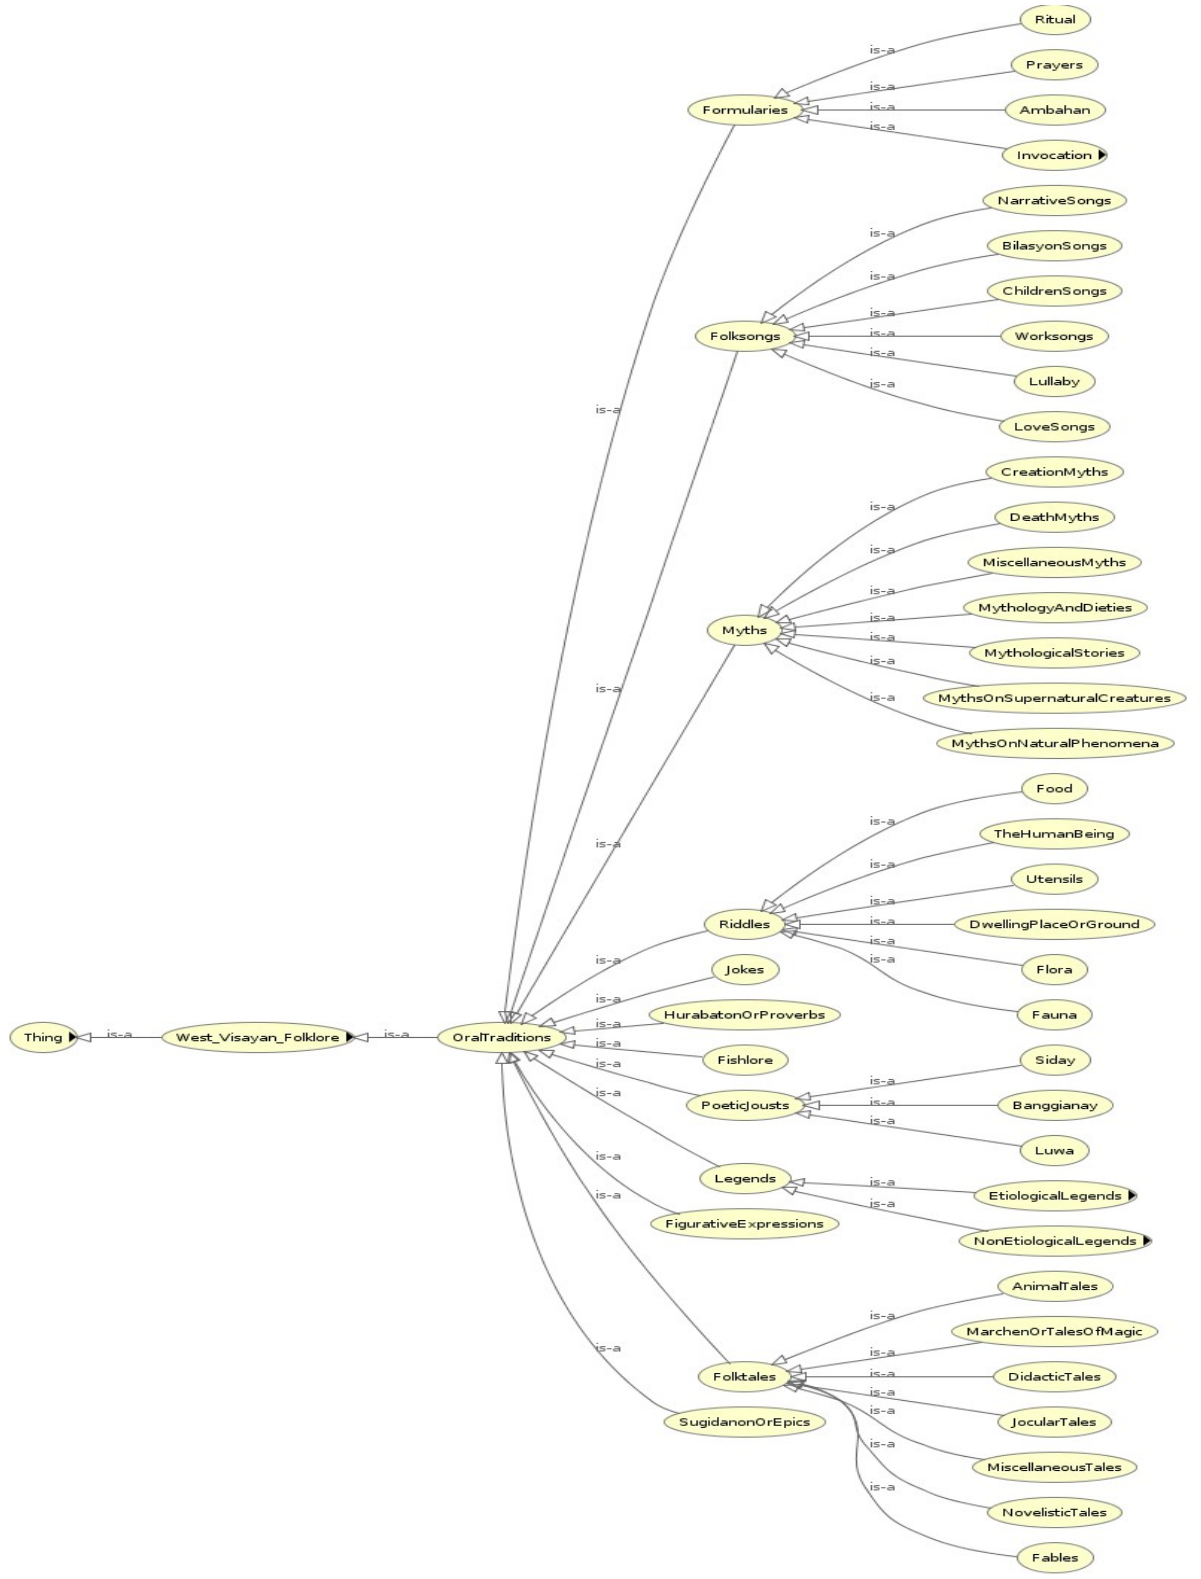
\includegraphics[width=\linewidth]{figures/Dimzon and Dimzon (2015) Ontology.png}
    \caption{Diagram of The Original Ontology by \protect\citeA{dimzon2015}}
    \label{fig:ontology diagram}
\end{figure}

As illustrated in Figure \ref{fig:ontology diagram}, the original ontology by \citeA{dimzon2015} does not contain story details but rather the classification of the different oral traditions found in the cultures of Western Visayas. This presents the knowledge gap that the researchers propose on exploring. Specifically, the ontology will be expanded with story elements for the Myths, Legends, and Folktales entities present in the current iteration of the ontology.

\begin{figure}[H]
    \centering
    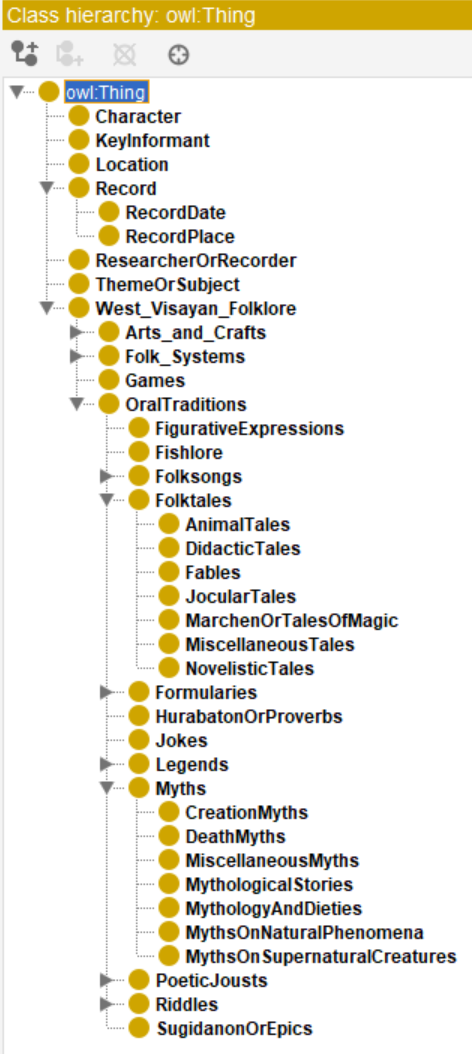
\includegraphics[width=0.5\linewidth]{figures/Class Hierarchy of Original Ontology.png}
    \caption{Class Hierarchy of Original Ontology}
    \label{fig:class hierarchy}
\end{figure}

Figure \ref{fig:class hierarchy} presents the class hierarchy of the objects in the original ontology as presented in Protege. Classes are categories or types of things in the ontology, representing a group of objects or individuals that share common characteristics. Instances of these classes are called individuals in Protege, representing a specific thing that belongs to the class. In the ontology enhancement phase, the researchers will introduce new classes in close guidance with literature experts. In the ontology expansion phase, the researchers will be populating relevant classes with new individuals.

\begin{figure}[H]
    \centering
    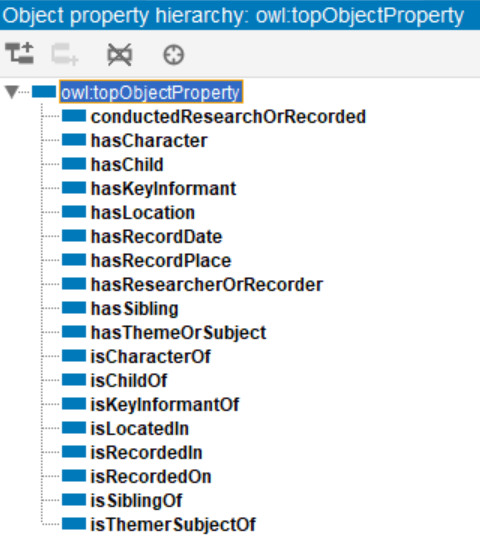
\includegraphics[width=0.5\linewidth]{figures/Object Property Hierarchy of Original Ontology.png}
    \caption{Object Property Hierarchy of Original Ontology}
    \label{fig:object property hierarchy}
\end{figure}

Figure \ref{fig:object property hierarchy} presents the hierarchy of the object properties in the original ontology as presented in Protege. Object properties define relationships between two individuals in the ontology, and are used to link classes or instances. In the ontology enhancement phase, the researchers will introduce new object properties to accommodate the new classes. In the ontology expansion phase, the researchers will encode relevant object properties that were present in the folk narratives.

\begin{figure}[H]
    \centering
    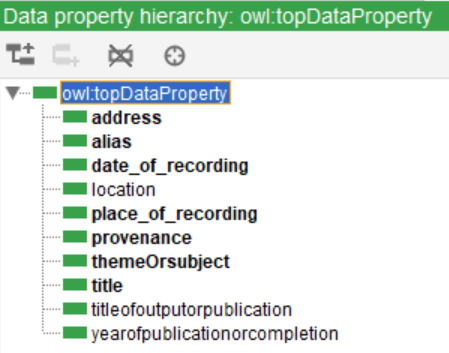
\includegraphics[width=0.5\linewidth]{figures/Data Property Hierarchy of Original Ontology.png}
    \caption{Data Property Hierarchy of Original Ontology}
    \label{fig:data property hierarchy}
\end{figure}

Figure \ref{fig:data property hierarchy} presents the hierarchy of the data properties in the original ontology as presented in Protege. Data properties define relationships between an individual and a literal value, such as a string, number, or date.  In the ontology enhancement phase, the researchers will introduce new data properties to accommodate the new classes. In the ontology expansion phase, the researchers will encode relevant data properties that were present in the reports papers of the folk narratives.


\subsection{Initial Data Gathering}

The researchers have contacted their contact person Prof. Dimzon on her collection of folk narratives. She gave a Terminal Report \citeA{dimzonmyths} on her completed project on collecting myths and legends from Western Visayas. It listed a total of 189 stories, 28 being myths and 161 being legends. Each folk narrative has already been categorized into their respective types, including etiological legends, non-etiological legends, and others. Below is a list of the different types of folk narratives collected, their subtypes, and their count.

\begin{enumerate}[label=\Roman*.]
\item Myths: 28
    \item Legends: 161
    \begin{enumerate} [label=\Alph*.]
        \item Etiological Legends: 69
        \begin{enumerate}[label=\roman*.]
            \item How Legends: 59
            \begin{enumerate}[label=\alph*.]
                \item Origin of Animals: 14
                \item Origin of plants and forms of plant life: 4
                \item How places and things got their names: 41
            \end{enumerate}
        \end{enumerate}
        \item NonEtiological Legends: 83
            \begin{enumerate}[label=\roman*.]
                \item Heroic Legends - great men, culture heroes: 18
                \item Religious/Saints Legends: 9
                \item Legends on Supernatural/Enchanted Beings: 56
            \end{enumerate}
        \item Others: 9
    \end{enumerate}
\end{enumerate}




\FloatBarrier

